\hypertarget{zegar_8cpp}{\section{Dokumentacja pliku prj/zegar.cpp}
\label{zegar_8cpp}\index{prj/zegar.\-cpp@{prj/zegar.\-cpp}}
}


Definicja metody Start.  


{\ttfamily \#include \char`\"{}zegar.\-hpp\char`\"{}}\\*
Wykres zależności załączania dla zegar.\-cpp\-:
\nopagebreak
\begin{figure}[H]
\begin{center}
\leavevmode
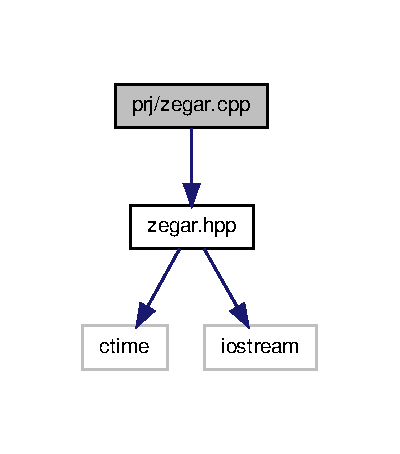
\includegraphics[width=192pt]{zegar_8cpp__incl}
\end{center}
\end{figure}


\subsection{Opis szczegółowy}
Definicja metody Start. Definicja metody Wynik.

Definicja metody Koniec.

Metoda, ktora powoduje start zegara.

Metoda, ktora powoduje stop zegara i oblicza czas.

Metoda, ktora wyswietla wynik. 

Definicja w pliku \hyperlink{zegar_8cpp_source}{zegar.\-cpp}.

